\documentclass[border=3pt]{standalone}
% Preâmbulo compartilhado pelos diagramas TikZ da aula 13 (SLAM com EKF)
\usepackage[T1]{fontenc}
\usepackage[utf8]{inputenc}
\usepackage{lmodern}
\usepackage{amsmath}
\usepackage{xcolor}
\usepackage{tikz}
\usetikzlibrary{arrows.meta,angles,quotes,decorations.pathmorphing,decorations.pathreplacing,calc,
                positioning,shapes.geometric,shapes.misc,backgrounds,fit,
                math}

% Paleta (mesma dos SVGs originais)
\definecolor{dblue}{HTML}{2A5B8C}
\definecolor{dorange}{HTML}{B3541E}
\definecolor{dgreen}{HTML}{4A7C59}
\definecolor{dred}{HTML}{9C4B4B}
\definecolor{dcream}{HTML}{F4F1EA}
\definecolor{dshade}{HTML}{DDD7C9}

% Função gaussiana (não normalizada por padrão de escala visual)
\pgfmathdeclarefunction{gauss}{3}{%
  \pgfmathparse{1/(#3*sqrt(2*pi))*exp(-((#1-#2)^2)/(2*#3^2))}%
}

% Estilos comuns (prefixo d... para não colidir com chaves internas do pgf)
\tikzset{
  >={Stealth[length=2mm]},
  dguide/.style={gray!55, dashed, line width=0.4pt},
  daxis/.style={gray!60, line width=0.7pt, ->},
  dbody/.style={fill=black!3, draw=black!80, line width=1pt},
  dacc/.style={draw=dblue, line width=1pt},
  dlbl/.style={black!55, font=\small},
  dsub/.style={black!45, font=\footnotesize},
  dstate/.style={circle, draw=black!80, fill=dcream, line width=1pt,
                 minimum size=17mm, font=\large, inner sep=1pt},
  dobs/.style={circle, draw=black!80, fill=dshade, line width=1pt,
               minimum size=14mm, font=\large, inner sep=1pt},
  dbox/.style={rounded corners=2pt, draw=black!80, fill=dcream, line width=1pt,
               align=center, inner sep=6pt},
  dop/.style={circle, draw=black!80, fill=white, line width=1pt,
              minimum size=6mm, inner sep=0pt, font=\small},
  dtrans/.style={->, dblue, line width=1pt},
  dmeas/.style={->, dorange, line width=1pt},
  dcurve/.style={line width=1pt, dblue},
  dcurveb/.style={line width=1.4pt, dorange},
}

\begin{document}
\hyphenpenalty=10000 \exhyphenpenalty=10000 \tolerance=9999 \emergencystretch=3em
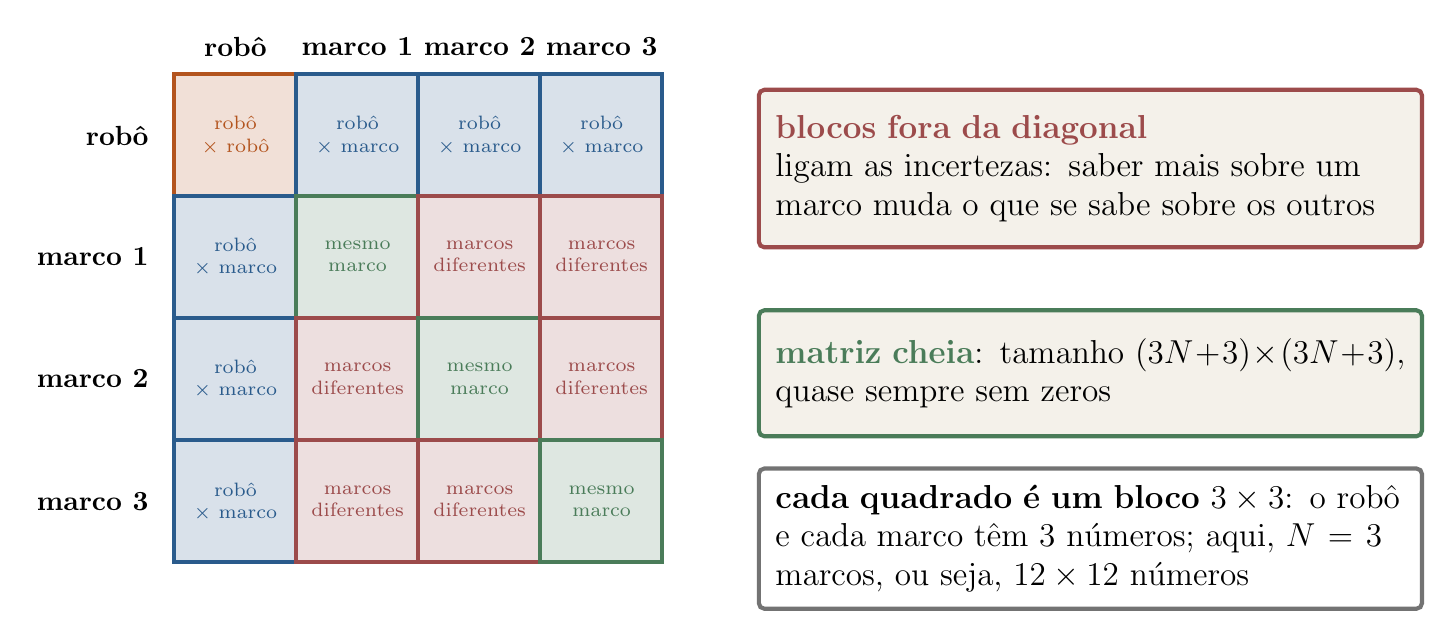
\begin{tikzpicture}[x=1cm,y=1cm]
\node[font=\normalsize\bfseries, anchor=east] at (-0.2,5.42) {robô};
\node[font=\normalsize\bfseries, rotate=0] at (0.78,6.55) {robô};
\node[font=\normalsize\bfseries, anchor=east] at (-0.2,3.88) {marco 1};
\node[font=\normalsize\bfseries, rotate=0] at (2.33,6.55) {marco 1};
\node[font=\normalsize\bfseries, anchor=east] at (-0.2,2.33) {marco 2};
\node[font=\normalsize\bfseries, rotate=0] at (3.88,6.55) {marco 2};
\node[font=\normalsize\bfseries, anchor=east] at (-0.2,0.77) {marco 3};
\node[font=\normalsize\bfseries, rotate=0] at (5.43,6.55) {marco 3};
\draw[dorange, fill=dorange!18, line width=1.3pt] (0.0,6.2) rectangle (1.55,4.65);
\node[font=\scriptsize, align=center, text=dorange] at (0.78,5.42) {robô\\$\times$ robô};
\draw[dblue, fill=dblue!18, line width=1.3pt] (1.55,6.2) rectangle (3.1,4.65);
\node[font=\scriptsize, align=center, text=dblue] at (2.33,5.42) {robô\\$\times$ marco};
\draw[dblue, fill=dblue!18, line width=1.3pt] (3.1,6.2) rectangle (4.65,4.65);
\node[font=\scriptsize, align=center, text=dblue] at (3.88,5.42) {robô\\$\times$ marco};
\draw[dblue, fill=dblue!18, line width=1.3pt] (4.65,6.2) rectangle (6.2,4.65);
\node[font=\scriptsize, align=center, text=dblue] at (5.43,5.42) {robô\\$\times$ marco};
\draw[dblue, fill=dblue!18, line width=1.3pt] (0.0,4.65) rectangle (1.55,3.1);
\node[font=\scriptsize, align=center, text=dblue] at (0.78,3.88) {robô\\$\times$ marco};
\draw[dgreen, fill=dgreen!18, line width=1.3pt] (1.55,4.65) rectangle (3.1,3.1);
\node[font=\scriptsize, align=center, text=dgreen] at (2.33,3.88) {mesmo\\marco};
\draw[dred, fill=dred!18, line width=1.3pt] (3.1,4.65) rectangle (4.65,3.1);
\node[font=\scriptsize, align=center, text=dred] at (3.88,3.88) {marcos\\diferentes};
\draw[dred, fill=dred!18, line width=1.3pt] (4.65,4.65) rectangle (6.2,3.1);
\node[font=\scriptsize, align=center, text=dred] at (5.43,3.88) {marcos\\diferentes};
\draw[dblue, fill=dblue!18, line width=1.3pt] (0.0,3.1) rectangle (1.55,1.55);
\node[font=\scriptsize, align=center, text=dblue] at (0.78,2.33) {robô\\$\times$ marco};
\draw[dred, fill=dred!18, line width=1.3pt] (1.55,3.1) rectangle (3.1,1.55);
\node[font=\scriptsize, align=center, text=dred] at (2.33,2.33) {marcos\\diferentes};
\draw[dgreen, fill=dgreen!18, line width=1.3pt] (3.1,3.1) rectangle (4.65,1.55);
\node[font=\scriptsize, align=center, text=dgreen] at (3.88,2.33) {mesmo\\marco};
\draw[dred, fill=dred!18, line width=1.3pt] (4.65,3.1) rectangle (6.2,1.55);
\node[font=\scriptsize, align=center, text=dred] at (5.43,2.33) {marcos\\diferentes};
\draw[dblue, fill=dblue!18, line width=1.3pt] (0.0,1.55) rectangle (1.55,-0.0);
\node[font=\scriptsize, align=center, text=dblue] at (0.78,0.77) {robô\\$\times$ marco};
\draw[dred, fill=dred!18, line width=1.3pt] (1.55,1.55) rectangle (3.1,-0.0);
\node[font=\scriptsize, align=center, text=dred] at (2.33,0.77) {marcos\\diferentes};
\draw[dred, fill=dred!18, line width=1.3pt] (3.1,1.55) rectangle (4.65,-0.0);
\node[font=\scriptsize, align=center, text=dred] at (3.88,0.77) {marcos\\diferentes};
\draw[dgreen, fill=dgreen!18, line width=1.3pt] (4.65,1.55) rectangle (6.2,-0.0);
\node[font=\scriptsize, align=center, text=dgreen] at (5.43,0.77) {mesmo\\marco};
\node[dbox, draw=dred, line width=1.5pt, text width=8.0cm, minimum height=2.0cm, font=\large, align=left, anchor=west] at (7.4,5.0) {\textbf{\textcolor{dred}{blocos fora da diagonal}}\\ ligam as incertezas: saber mais sobre um marco muda o que se sabe sobre os outros};
\node[dbox, draw=dgreen, line width=1.5pt, text width=8.0cm, minimum height=1.6cm, font=\large, align=left, anchor=west] at (7.4,2.4) {\textbf{\textcolor{dgreen}{matriz cheia}}: tamanho $(3N+3)\times(3N+3)$, quase sempre sem zeros};
\node[dbox, draw=black!55, fill=white, line width=1.5pt, text width=8.0cm, minimum height=1.6cm, font=\large, align=left, anchor=west] at (7.4,0.3) {\textbf{cada quadrado é um bloco $3\times 3$}: o robô e cada marco têm 3 números; aqui, $N=3$ marcos, ou seja, $12\times 12$ números};
\end{tikzpicture}
\end{document}
